\appendix
\section*{Appendix}
\section{Societal Impact}
In this paper, we quantify the influence of input features on the incurred bias/unfairness of the classifier on a dataset. This quantification facilitates our understanding of potential features or subsets of features attributing highly to the bias. This also allows us to understand the effect of the fairness enhancing algorithms in removing bias and their achievement/failure to do so. To the best of our understanding, this paper does not have any negative societal impact. 

\section{FIF as Difference of Conditional Variances: Proof of Theorem 1}\label{sec:proof_1}

\begin{theoremrep}[FIF as Difference of Conditional Variances]
	\label{lemma:fif_rep}
	Let $ V_{\mathbf{a}, \mathbf{S}} \triangleq \mathsf{Var}_{\nonsensitive_{\mathbf{S}}}[\widehat{Y} = 1|\sensitive = \mathbf{a}] $ be the decomposed conditional variance of the classifier's positive prediction for the sensitive group $ \sensitive = \mathbf{a} $, where features $ \nonsensitive_{\mathbf{S}} $ are jointly varied. Let $\mathbf{a}_{\max}$ and $\mathbf{a}_{\min}$ be the most and the least favored groups, respectively. Then, FIF of $ \nonsensitive_{\mathbf{S}} $ corresponding to statistical parity is
	\begin{equation}\tag{\ref{eq:fif_decompose}}
	w_{\mathbf{S}}  = \frac{V_{\mathbf{a}_{\max},\mathbf{S}} - V_{\mathbf{a}_{\min},\mathbf{S}}}{1 - (\Pr[\widehat{Y} = 1 |  \sensitive = \mathbf{a}_{\max}] + \Pr[\widehat{Y} = 1 |  \sensitive = \mathbf{a}_{\min}])},
	\end{equation}
	and FIFs defined by Equation~\eqref{eq:fif_decompose} satisfy Axiom~\ref{axm:additivity}.
\end{theoremrep}


\begin{proof}

Let $ B_{\mathbf{a}} \in \{0, 1\} $ be a Bernoulli random variable such that $ B_{\mathbf{a}} = 1 $ denotes the classifier predicting positive class $ \hat{Y} = 1 $ for an individual belonging to the sensitive group $ \sensitive = \mathbf{a} $, and $ B_{\mathbf{a}} = 0 $ denotes $ \hat{Y} = 0 $. Hence, if $ p_\mathbf{a} \triangleq \Pr[B_\mathbf{a} = 1] $, then $ p_\mathbf{a} $ is also the conditional probability of positive prediction of the classifier,  $ p_\mathbf{a} = \Pr[\hat{Y} = 1 |  \sensitive = \mathbf{a}] $. The variance of $ B_{\mathbf{a}} $ is computed as
\begin{align*}
	\mathsf{Var}[B_\mathbf{a}] = p_{\mathbf{a}}(1 - p_{\mathbf{a}}). 
\end{align*}

Now, we consider two Bernoulli random variables $ B_\mathbf{a} $ and $ B_\mathbf{a'} $ associated with two different sensitive groups $ \sensitive = \mathbf{a} $ and $ \sensitive = \mathbf{a}' $, respectively. The difference in variances between $ B_\mathbf{a} $ and $ B_\mathbf{a'} $ implies that
\begin{align*}
	\mathsf{Var}[B_\mathbf{a}] - \mathsf{Var}[B_\mathbf{a'}] &= p_{\mathbf{a}}(1 - p_{\mathbf{a}}) - p_{\mathbf{a'}}(1 - p_{\mathbf{a'}}) \\
	&= p_{\mathbf{a}} - p_{\mathbf{a}}^2 - p_{\mathbf{a'}} + p_{\mathbf{a'}}^2 \\ 
	&= (p_\mathbf{a} -  p_\mathbf{a'}) (1 - (p_\mathbf{a} + p_\mathbf{a'}))
\end{align*}

After reorganization, we express the difference in probabilities $ p_\mathbf{a} -  p_\mathbf{a'} $ as
\begin{align}
	\label{eq:sp_to_var}
	p_\mathbf{a} -  p_\mathbf{a'}  = \frac{	\mathsf{Var}[B_\mathbf{a}] - \mathsf{Var}[B_\mathbf{a'}]}{1 - (p_\mathbf{a} + p_\mathbf{a'})}
\end{align}




By setting $ \mathbf{a} = \mathbf{a}_{\max} $ and $ \mathbf{a'} = \mathbf{a}_{\min} $ in Equation~\eqref{eq:sp_to_var}, we express the statistical parity of the classifier in terms of the scaled difference in the conditional variance of the positive prediction of the classifier. 
\begin{align}
	f_{\mathsf{SP}}(\alg, \mathbf{D}) \triangleq p_{\mathbf{a}_{\max}} -  ~~p_{\mathbf{a}_{\min}}  &= \frac{	\mathsf{Var}[B_{\mathbf{a}_{\max}}] - \mathsf{Var}[B_{\mathbf{a}_{\min}}]}{1 - (p_{\mathbf{a}_{\max}} + p_{\mathbf{a}_{\min}})}\label{eq:sp_var_diff}\\
	&= \frac{	\mathsf{Var}[\hat{Y} = 1| \sensitive = \mathbf{a}_{\max}] - \mathsf{Var}[\hat{Y} = 1| \sensitive = \mathbf{a}_{\min}]}{1 - (p_{\mathbf{a}_{\max}} + p_{\mathbf{a}_{\min}})} \notag.
\end{align}

%The last inequality is obtained by the definition of $B_{\mathbf{a}}$.

Next, we apply variance decomposition (Equation~\eqref{eq:variance_decomposition_set_notation}) to estimate the influence of each $ \nonsensitive_{\mathbf{S}} $. From Equation~\eqref{eq:variance_decomposition_set_notation} in Section~\ref{sec:preliminaries}, we obtain that the variance of $ B_{\mathbf{a}} $ can be decomposed as 
\[ \mathsf{Var}[B_\mathbf{a}] = \sum_{\mathbf{S} \subseteq [\numnonsensitive] \setminus \emptyset} V_{\mathbf{a}, \mathbf{S}},\] 
where $ V_{\mathbf{a}, \mathbf{S}} $ denotes the decomposed variance of $ B_\mathbf{a} $ w.r.t.\ the features $ \nonsensitive_{\mathbf{S}} $ conditioned on the sensitive group $ \sensitive = \mathbf{a} $. 

Now, we apply variance decomposition on both $ \mathsf{Var}[B_{\mathbf{a}_{\max}}] $ and $ \mathsf{Var}[B_{\mathbf{a}_{\min}}] $ in Equation~\ref{eq:sp_var_diff} to obtain

\begin{align}
f_{\mathsf{SP}}(\alg, \mathbf{D}) & = \frac{\mathsf{Var}[B_{\mathbf{a}_{\max}}] - \mathsf{Var}[B_{\mathbf{a}_{\min}}]}{1 - (p_{\mathbf{a}_{\max}} + p_{\mathbf{a}_{\max}})}= \sum_{\mathbf{S} \subseteq [\numnonsensitive] \setminus \emptyset} \frac{V_{\mathbf{a}_{\max}, \mathbf{S}} - V_{\mathbf{a}_{\min}, \mathbf{S}}}{1 - (p_{\mathbf{a}_{\max}} + p_{\mathbf{a}_{\min}})} \label{eq:influence_value}
\end{align}
Finally, we estimate  the FIF of the subset of features $ \nonsensitive_{\mathbf{S}}  $ as 
\begin{align}
	w_{\mathbf{S}}  = \frac{V_{\mathbf{a}_{\max}, \mathbf{S}} - V_{\mathbf{a}_{\min}, \mathbf{S}}}{1 - (p_{\mathbf{a}_{\max}} + p_{\mathbf{a}_{\min}})}
\end{align} 
by separating the terms corresponding to $ \nonsensitive_{\mathbf{S}} $.

Following Equation~\eqref{eq:influence_value}, $	w_{\mathbf{S}} $ satisfies Axiom~\ref{axm:additivity} as $f_{\mathsf{SP}}(\alg, \mathbf{D}) = \sum_{\mathbf{S} \subseteq [\numnonsensitive] \setminus \emptyset} w_{\mathbf{S}} $.
\end{proof}


\section{A Smoothing Operator $\textsc{Smooth}$: Cubic Splines}
\label{sec:smoothing} 
In the $\textsc{LocalRegression}$ module of \framework{} (Line~\ref{algo_line:local_regression_start}--\ref{algo_line:local_regression_end}, Algorithm~\ref{algo:framework}), we use a smoothing operator $\textsc{Smooth}$ (Line~\ref{alg_line:backfitting_step}). In our experiments, \textit{we use cubic splines as the smoothing operator}. Here, we elucidate the technical details of cubic splines.

In interpolation problems, a B-spline of order $ n $ is traditionally used to smoothen the intersection of piecewise interpolators~\cite{schumaker2007spline}. A B-spline of degree $n$ is a piecewise polynomial of degree $ n - 1 $ defined over a variable $ X $. Each piecewise term is computed on local points and is aggregated as a global curve smoothly fitting the data. The values of $ X $ where the polynomial pieces meet together are called knots, and are denoted by $\{ \dots, t_0, t_1, t_2, \dots\} $. 

Let $ B_{r, n}(X) $ denote the basis function for a B-spline of order $ n $, and $ r $ is the index of the knot vector. According to Carl de Boor~\cite{de1971subroutine}, $ B_{r,1}(X) $, for $ n = 1 $, is defined as
\begin{align*}
B_{r,1}(X) = 
\begin{cases}
0 &\text{ if } X < t_r \text{ or } X \ge t_{r+1},\\
1 &\text{ otherwise}
\end{cases}
\end{align*}

This definition satisfies $ \sum_i B_{r, 1}(X) = 1 $. The higher order basis functions are defined recursively as
\begin{align*}
	B_{r, n + 1}(X) = p_{r, n}(X)B_{r, n}(X) + (1 - p_{r + 1, n}(X))B_{r + 1, n}(X),
\end{align*}
where 
\begin{align*}
p_{r,n}(X) = 
\begin{cases}
\frac{X - t_r}{t_{r + n} - t_r} &\text{ if } t_{r + n} \ne t_r,\\
0 &\text{ otherwise.}
\end{cases}
\end{align*}


In this paper, we consider cubic splines with the basis function $ B_{r,4}(X) $ that constitutes a B-spline of degree $ 3 $. This polynomial has $ C^2 $ continuity, i.e. for each piecewise term, derivatives up to the second order are zero at the endpoints of each interval in the knot vector. We estimate component functions $ \function_{\mathbf{a}, \mathbf{S}} $'s with the basis function $ B_{r,4}(\mathbf{X})  $ of cubic splines~\cite{li2010global}, as shown in Equation~\eqref{eq:cubic_splines}.  
\begin{align}\label{eq:cubic_splines}
\begin{split}
&\function_{\mathbf{a}, \{i\}} (\mathbf{X}_{\{i\}}) \approx \sum_{r=-1}^{m+1}\alpha_r^iB_{r,n}(\mathbf{X}_{\{i\}})\\
&\function_{\mathbf{a}, \{i, j\}} (\mathbf{X}_{\{i, j\}}) \approx \sum_{p=-1}^{m+1}\sum_{q=-1}^{m+1}\beta_{pq}^{ij}B_p(\mathbf{X}_{\{i\}})B_q(\mathbf{X}_{\{j\}})\\
&\function_{\mathbf{a}, \{i, j, k\}} (\mathbf{X}_{\{i, j, k\}}) \approx \sum_{p=-1}^{m+1}\sum_{q=-1}^{m+1}\sum_{r=-1}^{m+1}\gamma_{pqr}^{ijk}B_p(\mathbf{X}_{\{i\}})B_q(\mathbf{X}_{\{j\}})B_{r,n}(\mathbf{X}_{\{j\}})
\end{split}
\end{align}

Here, $ m $ is the number of knots. We learn the coefficients $ \alpha, \beta, \gamma $ using the backfitting algorithm (Line~\ref{algo_line:local_regression_start}--\ref{algo_line:local_regression_end}, Algorithm~\ref{algo:framework}). 

\begin{comment}
\paragraph{Kernel Smoothing.}
Kernel smoother estimates a real-valued function $ \function : \mathbb{R}^k \rightarrow \mathbb{R} $ as the weighted average of neighboring observed data. The weight is defined by the kernel such that closer points are given higher weights. The estimated function is smooth, where the level of smoothness is specified by a single parameter. Let $ k_{h_\lambda}(\mathbf{X}_0, \mathbf{X}) $ be a kernel defined by
\[
k_{h_\lambda}(\mathbf{X}_0, \mathbf{X}) = D\Big(\frac{||\mathbf{X}_0, \mathbf{X}||}{h_\lambda(\mathbf{X}_0)}\Big)
\]

where: 
\begin{itemize}
	\item $ \mathbf{X}_0, \mathbf{X} \in \mathbb{R}^k $
	\item $ ||\cdot|| $ is Euclidean norm
	\item $ h_\lambda(\mathbf{X}_0) $ is a parameter known as kernel radius
	\item $ D(t) $ is a positive real-valued function, whose value is decreasing (or not increasing) for the increasing distance $ t $
\end{itemize}
Popular kernels used for smoothing include parabolic, tricube, and Gaussian kernels. Popular kernel smoothers are Gaussian kernel smoother, nearest neighbor smoother, kernel average smoother, local linear or polynomial regression.

\end{comment}

%\clearpage
\section{Experimental Evaluations}\label{sec:additional_experiments}


\subsection{Experimental Setup}
We conduct experiments on Red Hat Enterprise Linux Server release 6.10 (Santiago) with $ \text{E}5-2690 \text{ v}3 $ CPU and $ 8 $GB of RAM. Since our objective is to compute FIFs for any classifier, we do not perform any tuning of hyper-parameters during training. We use the default hyper-parameter choices available in Scikit-learn~\cite{scikit-learn}. The only parameter that we choose in {\framework} is the maximum order of intersectionality, namely $ \lambda $. We present the ablation study w.r.t.\ $ \lambda $ in Appendix~\ref{sec:ablation}.


\subsection{Runtime of {\framework}} 
In Figure~\ref{fig:runtime}, we report the runtime of {\framework} in computing FIFs (with $ \lambda = 2 $) for different group fairness metrics on four classifiers and five datasets. The dimension of the dataset, measured by the number of samples and the number of features, is a key factor for runtime. For example, Adult dataset has the maximum number of samples ($ = 26048 $) compared to other datasets. In contrast, German dataset has the maximum features ($ = 26 $). Consequently, {\framework} requires more runtime in both Adult and German dataset compared to others. However, \emph{in all datasets, FIF computation takes at most $ 25 $ seconds, that demonstrates the efficiency of {\framework} in practical fairness problems.}

\begin{figure}[h!]
	\centering
	\subfloat[Statistical parity]{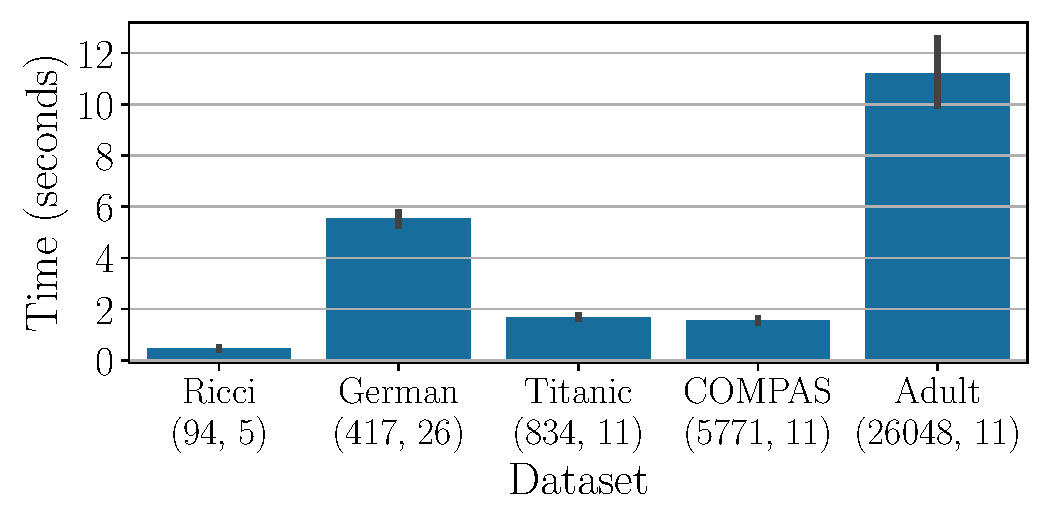
\includegraphics[scale=0.39]{figures/sp_train_time_detailed_fairXplainer_only}}
	\subfloat[Equalized odds]{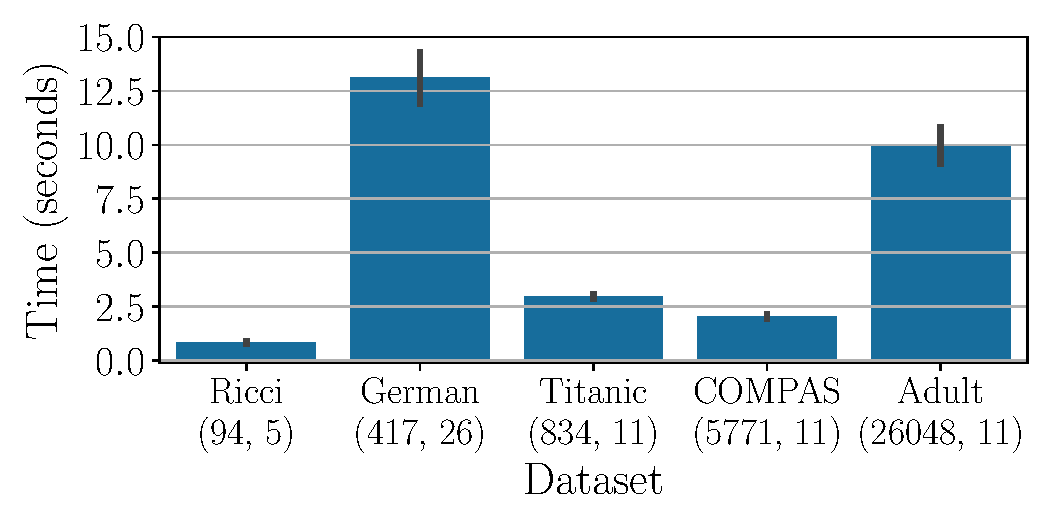
\includegraphics[scale=0.39]{figures/eo_train_time_detailed_fairXplainer_only}}\\
	\subfloat[Predictive parity]{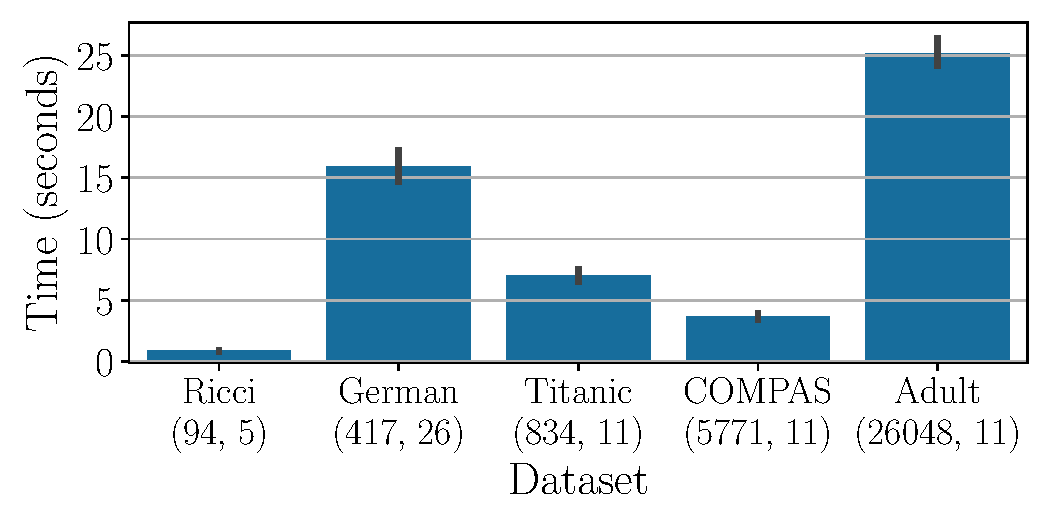
\includegraphics[scale=0.39]{figures/suff_train_time_detailed_fairXplainer_only}}
	\caption{Runtime of {\framework} (in seconds) for computing FIFs in different datasets. For each dataset, we mention its dimension as a tuple (\# sample, \# features) in the xticks. As the dimension increases, we observe higher runtime of {\framework}.}\label{fig:runtime}\vspace*{-1em}
\end{figure}

\subsection{Ablation Study: Effect of Maximum Order of Intersectionality $ \lambda $}\label{sec:ablation} 
We test the effect of $ \lambda \in \{1, 2, 3\} $ on the runtime of {\framework}. For each $ \lambda $, we consider $ 540 $ fairness instances ($ 5 $ datasets with $ 27 $ different combinations of sensitive features $ \times $ $ 5 $-fold cross validation $ \times $ $ 4 $ classifiers). We plot the corresponding results in the cumulative distribution plot of  Figure~\ref{fig:varying_max_order}. Here, $ X $-axis denotes the runtime (in seconds) and $ Y $-axis denotes the total number of solved instances, i.e. a point $ (x,y) $ denotes that $ y $ number of instances are solved within $ x $ seconds. 

As we increase from $ \lambda = 1 $ to $ \lambda = 2 $ and then to $ \lambda = 3 $, {\framework} requires around $ 0.5 $ and $ 2 $ orders of magnitude more runtime, respectively, to solve the equal number of instances. This is due to the fact that with increase in $ \lambda $, there is a combinatorial explosion in the number of component functions in the backfitting algorithm. Thus, \emph{computing higher-order FIFs requires a higher runtime of {\framework}}. 

\begin{figure}[t!]
	\centering
	{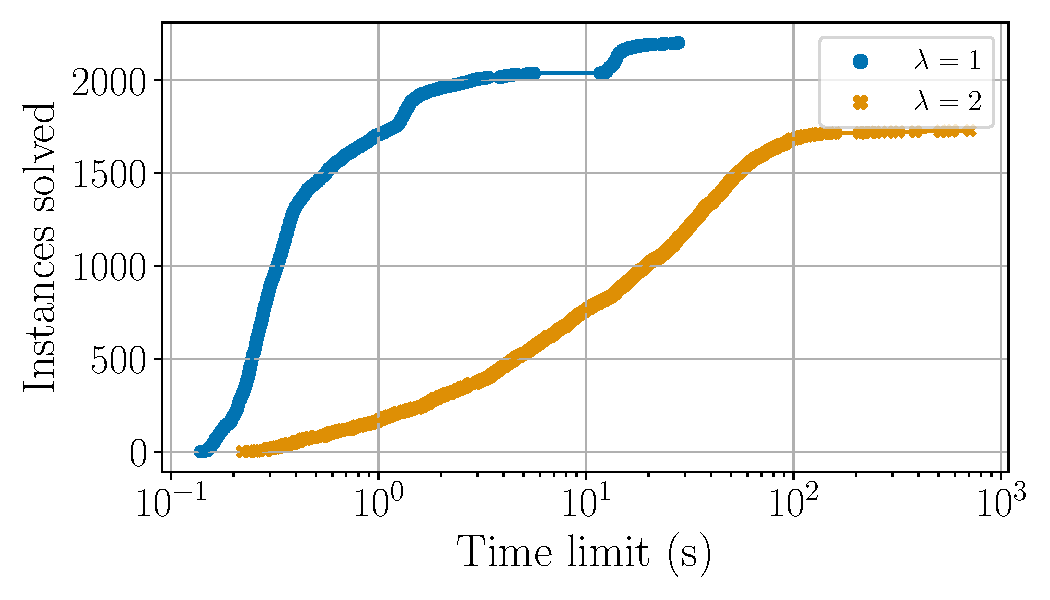
\includegraphics[scale=0.38]{figures/vary_max_order_train}}
	%	\subfloat[]{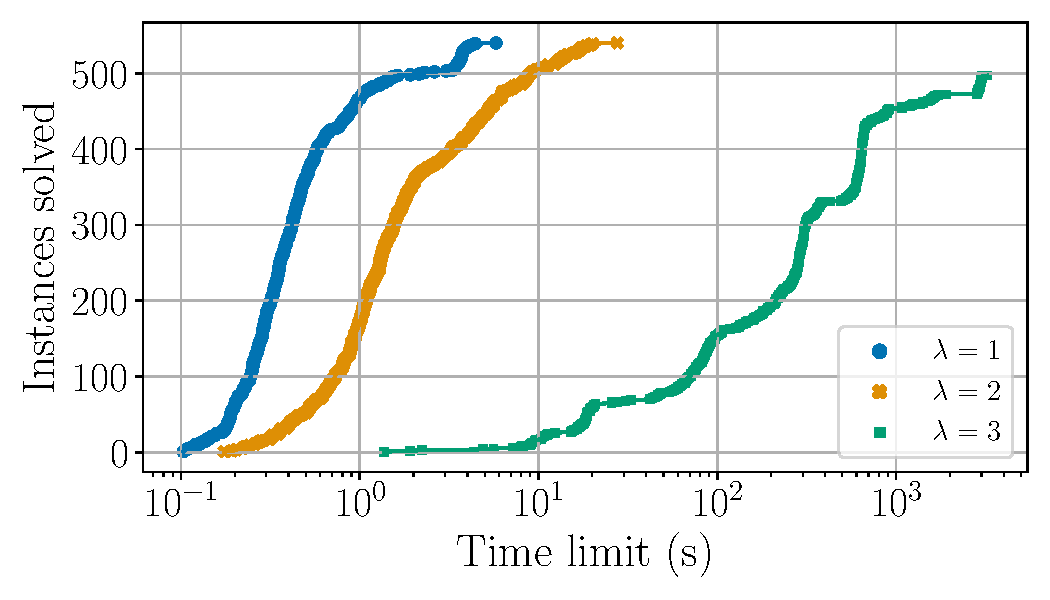
\includegraphics[scale=0.4]{figures/vary_max_order_test}}	
	\caption{Effect on runtime while varying max-order $ \lambda $ in {\framework}. Higher $ \lambda $ incurs more a computational effort, hereby solving less fairness instances within the same time limit.}\label{fig:varying_max_order}
\end{figure}


\subsection{Accuracy in Estimating Different Fairness Metrics}
We compare and evaluate the accuracies of {\framework} and SHAP in estimating a fairness metric, computed as the sum of FIFs (Axiom~\ref{axm:additivity}). We illustrate the results with a scatter-plot in Figure~\ref{fig:accuracy_scatter_plot}. In the plot, each dot represents the estimation of a fairness metric on a dataset and a classifier. 

The majority of dots for {\framework} are on the line connecting $ (0, 0) $ to $ (1, 1) $  in Figure~\ref{fig:accuracy_scatter_plot}. This implies that the estimation of {\framework} is significantly accurate. Interestingly, error rarely occurs in {\framework} due to the degenerate cases mentioned in Section~\ref{sec:fifs}. 
In contrast, SHAP often computes a metric inaccurately, thereby showing the drawback of applying a local explanation approach for FIF computation. \emph{Thus, {\framework} is significantly more accurate than SHAP in computing FIFs and the corresponding fairness metrics.}


\begin{figure}[t!]\vspace*{-1em}
	\centering
	\subfloat[Statistical parity]{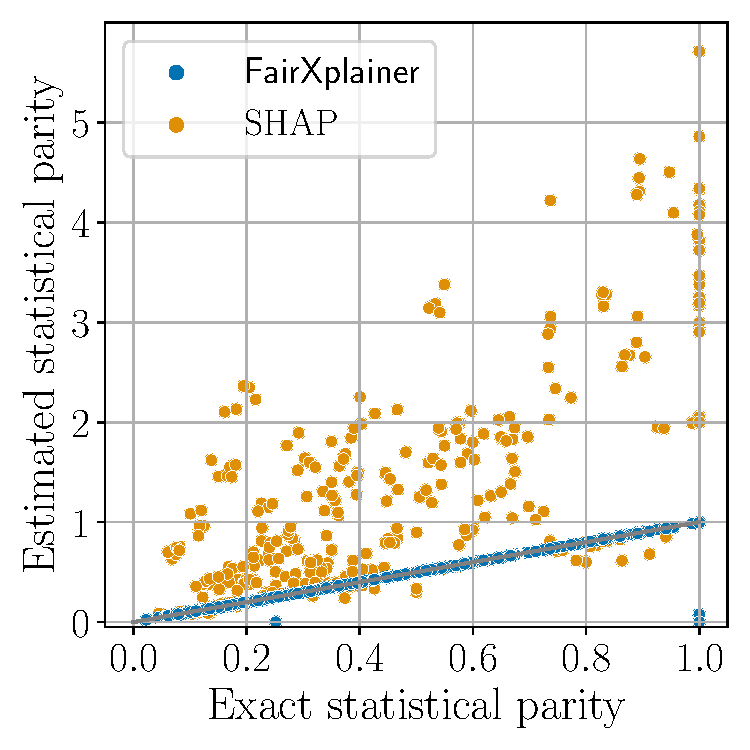
\includegraphics[scale=0.35]{figures/scatter_plot_sp_train_accuracy}}
	\subfloat[Equalized odds]{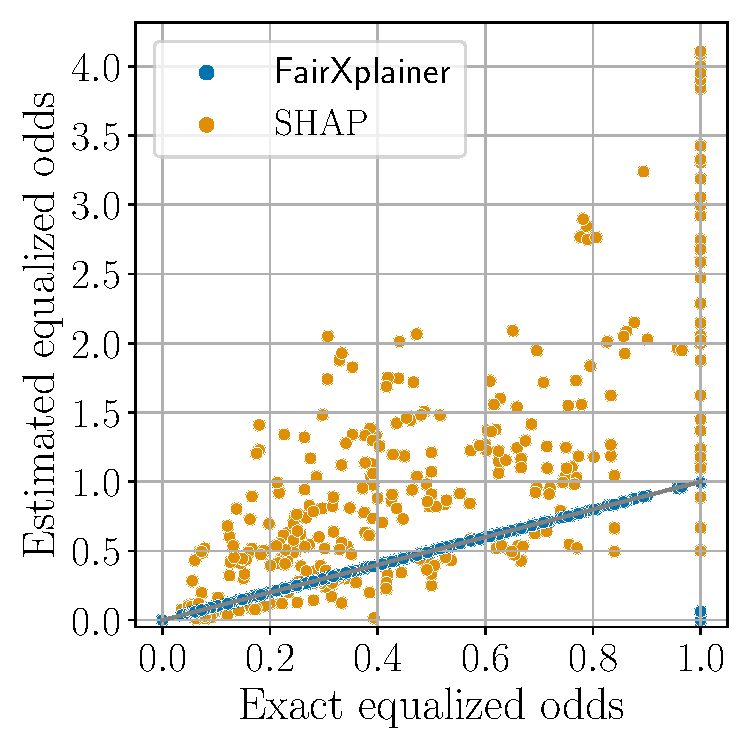
\includegraphics[scale=0.35]{figures/scatter_plot_eo_train_accuracy}}
	\subfloat[Predictive parity]{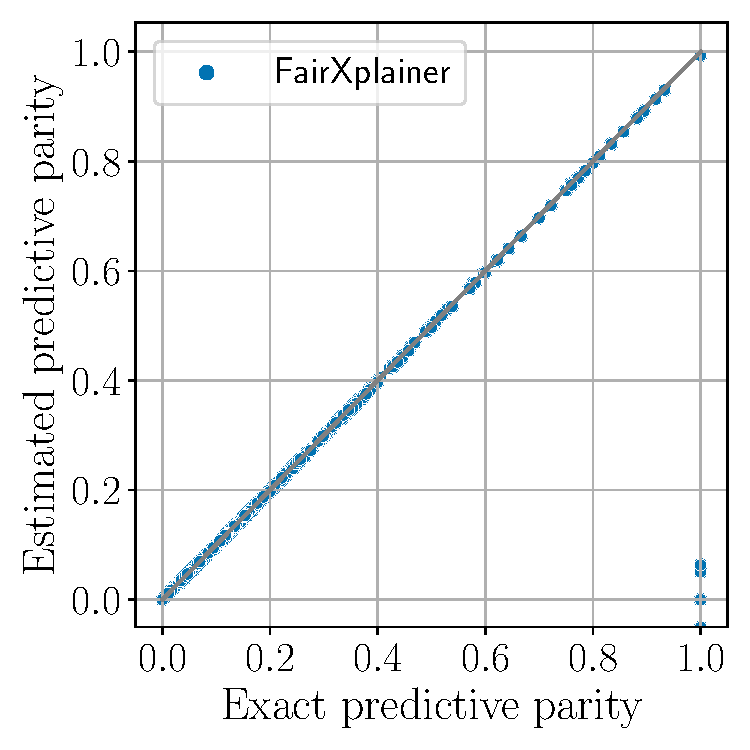
\includegraphics[scale=0.35]{figures/scatter_plot_suff_train_accuracy}}
	\caption{Comparison between the estimated and exact value of a fairness metric, computed as the sum of FIFs according to Axiom~\ref{axm:additivity}. Results are presented separately for {\framework} and SHAP. Each dot represents the result for a fairness metric, carried over multiple datasets and classifiers. Ideally, if a dot lies on the line connecting $ (0,0) $ to $ (1,1) $, it denotes a correct fairness estimate. {\framework} demonstrates significantly better accuracy of estimation than SHAP. For predictive parity metric, only {\framework} allows associated FIFs computation.}
	\label{fig:accuracy_scatter_plot}
\end{figure}



\subsection{FIF of Different Datasets}
We deploy a neural network ($ 3 $ hidden layers, each with $ 2 $ neurons, L$ 2 $ penalty regularization term as $ 10^{-5} $, a constant learning rate as $ 0.001 $) on different datasets, namely Adult, Ricci, and Titanic, and demonstrate the corresponding FIFs in Figures~\ref{fig:individual_vs_intersectional_influence_adult},~\ref{fig:individual_vs_intersectional_influence_ricci}, and \ref{fig:individual_vs_intersectional_influence_titanic}, respectively. In all the figures, both individual and intersectional FIFs depict the sources of bias more clearly than individual FIFs alone, as argued in Section~\ref{sec:experiments}. 


\textbf{In Adult dataset,} the classifier predicts whether an individual earns more than $ \$50 $k per year or not, where `race' and `sex' are sensitive features. We observe that the trained network is unfair and it demonstrates statistical parity as $ 0.23 $. As we analyze FIFs,  \textit{education number}, \textit{age}, and \textit{capital gain/loss} are key features responsible for the bias. Unlike COMPAS dataset (Figure~\ref{fig:individual_and_intersectional_fifs}), there does not exist any feature or subset of features in Adult dataset that potentially reduces the bias.

\begin{figure}[!t]
	\begin{minipage}{0.45\textwidth}
		\centering
		\subfloat[Individual FIFs]{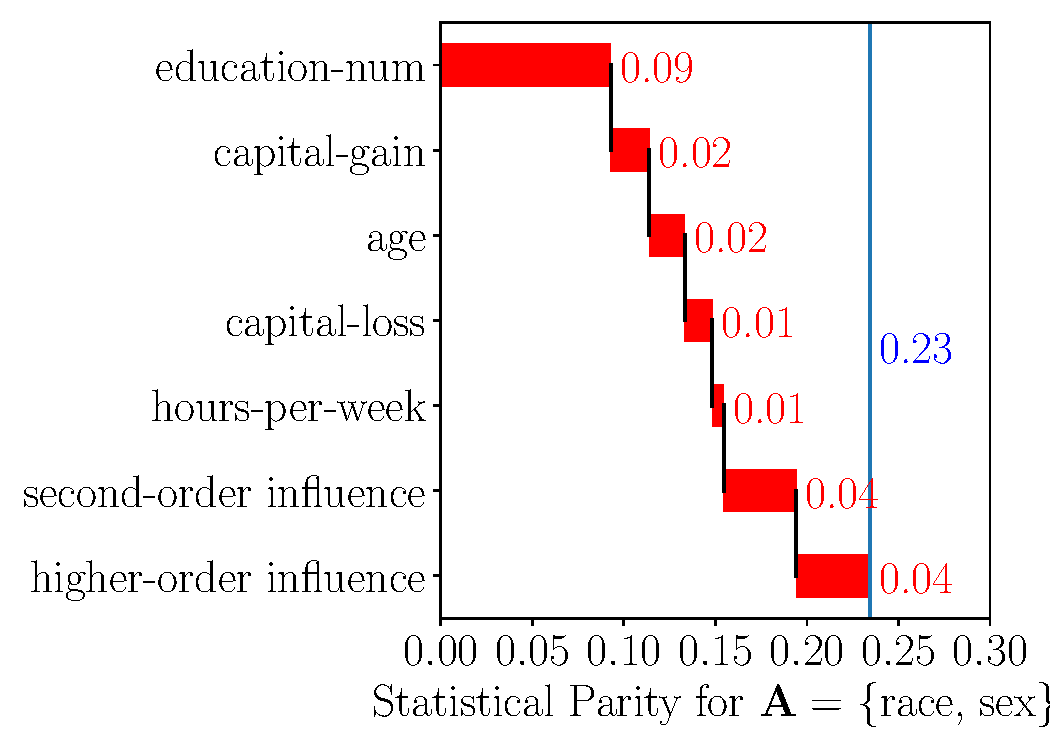
\includegraphics[scale=0.35]{figures/adult_feature_weight_unsorted}\label{fig:individual_fifs_adult}}
	\end{minipage}
	\begin{minipage}{0.5\textwidth}
		\centering
		\subfloat[Individual and intersectional FIFs]{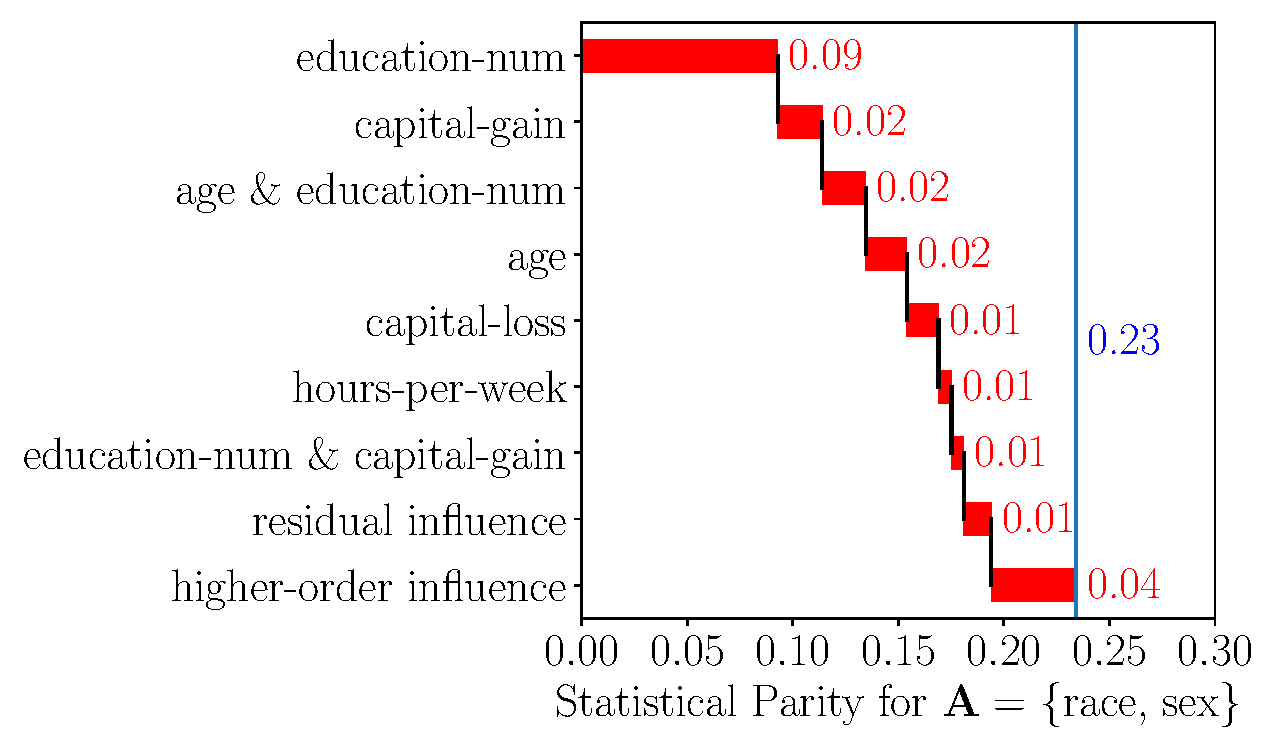
\includegraphics[scale=0.35]{figures/adult_feature_weight}\label{fig:individual_and_intersectional_fifs_adult}}
	\end{minipage}
	\vspace{-0.2em}
	\caption{FIFs for Adult dataset on explaining statistical parity. }\label{fig:individual_vs_intersectional_influence_adult}
	
\end{figure}



\textbf{In Ricci dataset,} the classification task  is to predict whether a firefighter obtains promotion or not in New Haven, Connecticut administered exams. We consider `race' as the sensitive feature for this experiment. We observed that the classifier has statistical parity of $ 0.3 $ based on the race of a person. In the computed FIFs, the \textit{combined score} and \textit{desired position} of a person increases bias, whereas written exam score reduces bias while interacting with other features. In addition, the higher order influences demonstrate a higher value (FIF $ = 0.26 $), meaning that the features are highly correlated and act in favor of bias.

\begin{figure}[h!]
	\begin{minipage}{0.45\textwidth}
		\centering
		\subfloat[Individual FIFs]{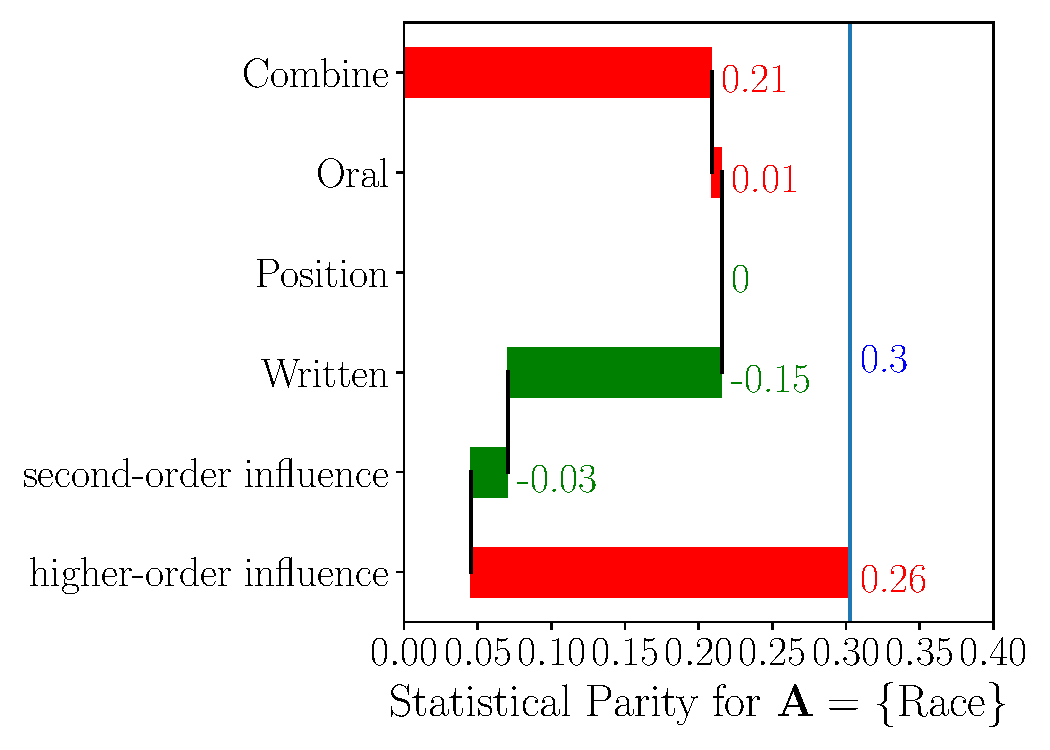
\includegraphics[scale=0.35]{figures/ricci_feature_weight_unsorted}\label{fig:individual_fifs_ricci}}
	\end{minipage}
	\begin{minipage}{0.5\textwidth}
		\centering
		\subfloat[Individual and intersectional FIFs]{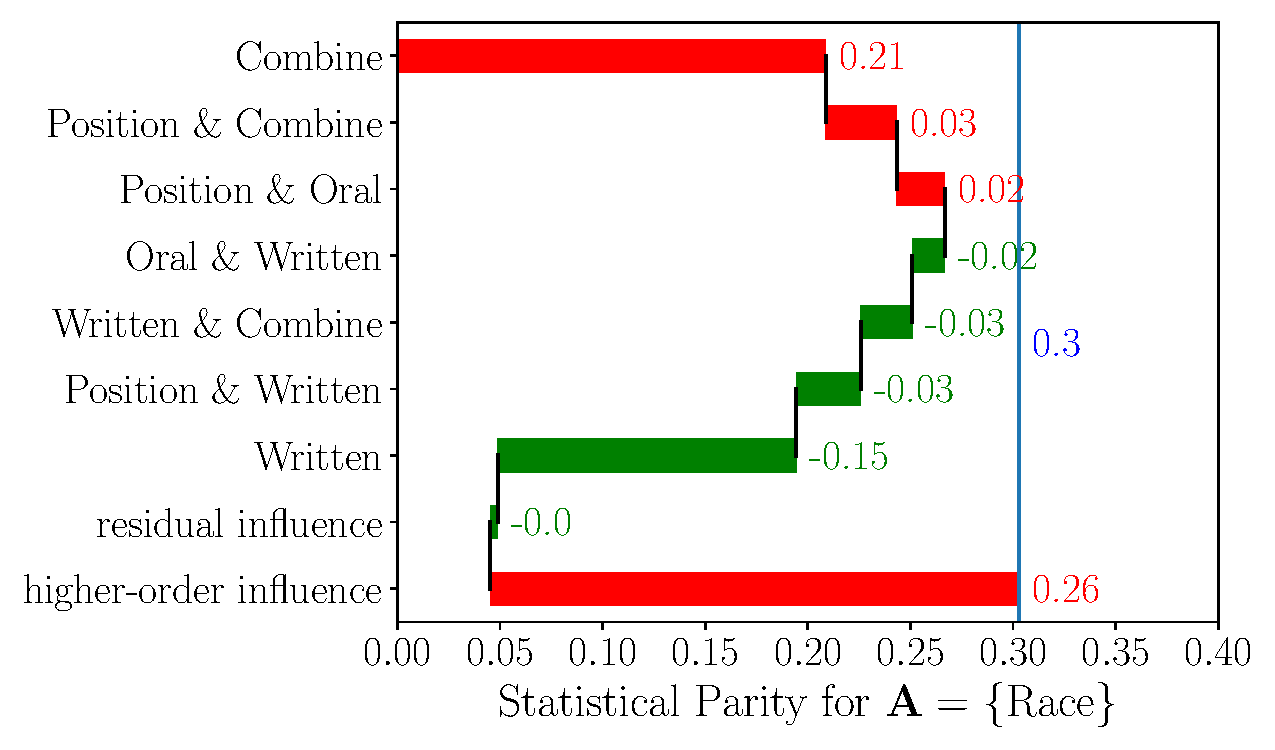
\includegraphics[scale=0.35]{figures/ricci_feature_weight}\label{fig:individual_and_intersectional_fifs_ricci}}
	\end{minipage}
	\vspace{-0.2em}
	\caption{FIFs for Ricci dataset on explaining statistical parity.}\label{fig:individual_vs_intersectional_influence_ricci}
	
\end{figure}

\textbf{In Titanic dataset,} the neural network predicts whether a person survives the Titanic shipwreck or not. In this experiment, we consider the `sex' of a person as a sensitive feature and observe that the classifier is highly unfair (statistical parity as $ 0.83 $) on the basis of `sex'. In the computed FIFs, most of the features except the \textit{passenger class} and the \textit{age} of a person increases the bias of the classifier.

\begin{figure}[h!]
	\begin{minipage}{0.45\textwidth}
		\centering
		\subfloat[Individual FIFs]{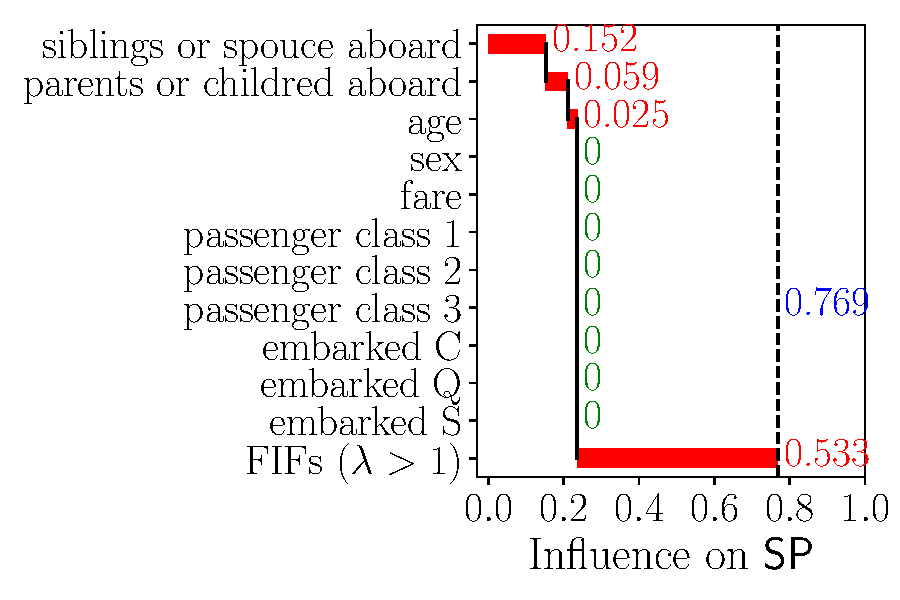
\includegraphics[scale=0.35]{figures/titanic_feature_weight_unsorted}\label{fig:individual_fifs_titanic}}
	\end{minipage}
	\begin{minipage}{0.5\textwidth}
		\centering
		\subfloat[Individual and intersectional FIFs]{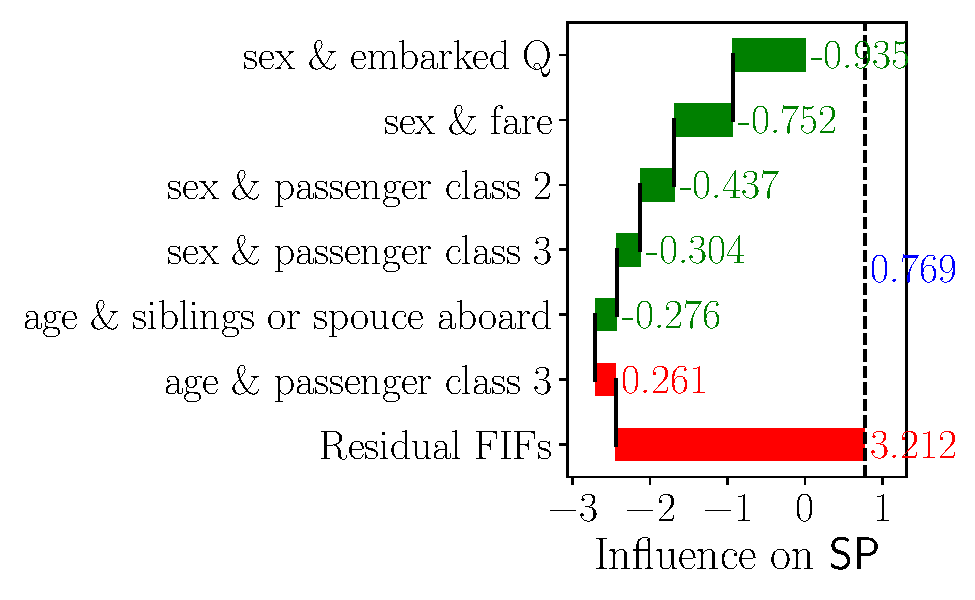
\includegraphics[scale=0.35]{figures/titanic_feature_weight}\label{fig:individual_and_intersectional_fifs_titanic}}
	\end{minipage}
	\vspace{-0.2em}
	\caption{FIFs for Titanic dataset on explaining statistical parity.}\label{fig:individual_vs_intersectional_influence_titanic}
	
\end{figure}